\documentclass[a4paper,11pt]{article}
\usepackage[margin=2.5cm]{geometry}
\usepackage{amsmath,amssymb,booktabs,graphicx,hyperref,xcolor,natbib}
\bibliographystyle{plainnat}

\title{VLOM Blend Weight Analysis:\\Optimal SED-Perch Fusion via LB Trend Modeling}
\author{Tom \\ Realtek Semiconductor Corp.}
\date{BirdCLEF+ 2026 --- April 2026}

\begin{document}
\maketitle

\begin{abstract}
We analyze the Variance-weighted Log-Odds Mean (VLOM) blend between Sound Event Detection (SED) and Perch foundation model predictions.
Through empirical leaderboard experiments and cross-validation EDA, we find that $w_\text{SED}=0.70$, $w_\text{Perch}=0.30$ is optimal (LB 0.943),
and identify a fundamental \emph{CV-LB inversion}: cross-validation strongly favors Perch-heavy blends ($w_\text{SED}=0.50$ achieves CV 0.990),
while the leaderboard rewards SED-heavy blends.
We explain this paradox through per-taxonomy analysis and infer characteristics of the hidden test distribution.
\end{abstract}

\section{Introduction}

The final prediction in our BirdCLEF+ 2026 pipeline combines two independent scoring branches via VLOM:
\begin{equation}
\hat{y}_\text{final} = \sigma\left(w_\text{SED} \cdot \text{logit}(\hat{y}_\text{SED}) + w_\text{Perch} \cdot \text{logit}(\hat{y}_\text{Perch})\right)
\end{equation}
where $w_\text{SED} + w_\text{Perch} = 1$.
The SED branch is a 3-model ONNX ensemble (EfficientNet-B0 R12 fold0 + PVT-v2-B0 R5 fold2 + B0 R6 fold3),
and the Perch branch is a Perch v2 foundation model with fine-tuned probe and ProtoSSM post-processing.

\section{Leaderboard Results}

\begin{table}[h]
\centering
\caption{VLOM weight experiments on Kaggle public leaderboard.}
\begin{tabular}{ccc}
\toprule
$w_\text{SED}$ & $w_\text{Perch}$ & LB Score \\
\midrule
0.70 & 0.30 & \textbf{0.943} \\
0.75 & 0.25 & 0.942 \\
0.50 & 0.50 & 0.937 \\
0.90 & 0.10 & 0.928 \\
\bottomrule
\end{tabular}
\label{tab:lb}
\end{table}

The optimal blend is $w_\text{SED}=0.70$: heavy enough to leverage SED's superior temporal resolution,
but retaining 30\% Perch contribution as a ``safety net'' for species where SED is weak.

\section{The CV-LB Inversion}

\subsection{Cross-Validation Favors Perch}

On 739 labeled soundscape windows (66 files), the CV AUC shows the \emph{opposite} trend from LB:

\begin{table}[h]
\centering
\caption{CV AUC (macro-averaged) at different VLOM weights, on 739 labeled windows.}
\begin{tabular}{ccc}
\toprule
$w_\text{SED}$ & CV AUC & LB \\
\midrule
0.50 & \textbf{0.9897} & 0.937 \\
0.55 & 0.9885 & --- \\
0.60 & 0.9873 & --- \\
0.65 & 0.9860 & --- \\
\textbf{0.70} & 0.9842 & \textbf{0.943} \\
0.75 & 0.9815 & 0.942 \\
0.80 & 0.9784 & --- \\
0.90 & 0.9710 & 0.928 \\
\midrule
SED only & 0.9594 & --- \\
Perch only & \textbf{0.9918} & --- \\
\bottomrule
\end{tabular}
\label{tab:cv}
\end{table}

\textbf{Key paradox}: Perch solo (0.9918) far exceeds SED solo (0.9594) on CV,
and lower $w_\text{SED}$ consistently gives higher CV AUC.
Yet on LB, $w_\text{SED}=0.70$ beats $w_\text{SED}=0.50$ by +0.006.

\subsection{Per-Taxonomy Explanation}

Solo model AUC by taxonomic class reveals the source:

\begin{table}[h]
\centering
\caption{Per-taxonomy solo AUC on labeled soundscapes.}
\begin{tabular}{lcccc}
\toprule
Class & \# Species & SED AUC & Perch AUC & Winner \\
\midrule
Aves & 28 & 0.9510 & 0.9929 & Perch \\
Amphibia & 17 & 0.9654 & 0.9865 & Perch \\
Insecta & 25 & 0.9742 & 0.9944 & Perch \\
Mammalia & 4 & 0.9025 & 0.9955 & Perch \\
\bottomrule
\end{tabular}
\label{tab:taxonomy}
\end{table}

\textbf{Perch dominates every single taxonomy on our labeled data.}
This is because our 66 labeled soundscapes are a small, potentially biased sample.
Perch v2 was pre-trained on massive bird call datasets and has excellent priors for the specific species present in our labeled set.

\subsection{Why LB Disagrees}

The hidden test set likely differs from our labeled soundscapes in several ways:
\begin{enumerate}
\item \textbf{More diverse acoustic conditions}: environmental noise, equipment variation, overlapping species --- where SED's mel-spectrogram training generalizes better than Perch's fixed embeddings.
\item \textbf{Different species distribution}: the 66 labeled soundscapes cover only 75/234 species. The remaining 159 species may have different SED-Perch relative strengths.
\item \textbf{Temporal structure}: SED processes 20s clips with attention-based temporal pooling; Perch processes 5s windows independently. Complex temporal patterns (calls with pauses, duets) favor SED.
\item \textbf{Confidence calibration}: Perch outputs well-calibrated probabilities for known species but may be overconfident on ambiguous cases. SED's lower confidence (mean=0.068 vs Perch's 0.039) paradoxically provides better separation at the LB AUC metric.
\end{enumerate}

\section{Per-Class Analysis: Why 0.70 Beats 0.75}

At the per-class level, \textbf{all 26 classes with measurable difference favor 0.70 over 0.75}; zero classes favor 0.75.

\begin{table}[h]
\centering
\caption{Top classes where 0.70/0.30 outperforms 0.75/0.25.}
\small
\begin{tabular}{llcccc}
\toprule
Species & Class & AUC(0.70) & AUC(0.75) & $\Delta$ \\
\midrule
strher2 & Aves & 0.5909 & 0.4763 & +0.115 \\
516975 & Mammalia & 0.9763 & 0.9645 & +0.012 \\
1491113 & Amphibia & 0.9173 & 0.9112 & +0.006 \\
74113 & Mammalia & 0.9980 & 0.9932 & +0.005 \\
47158son10 & Insecta & 0.9736 & 0.9688 & +0.005 \\
\bottomrule
\end{tabular}
\label{tab:perclass}
\end{table}

The largest effect is on \texttt{strher2} (Striated Heron), where reducing Perch weight from 0.30 to 0.25 causes a 0.115 AUC drop.
This is a species where SED has low confidence (near-random) and Perch provides the critical signal ---
at 0.25 Perch weight, the Perch signal is too attenuated to overcome SED's noise.

\section{Calibration Analysis}

\begin{table}[h]
\centering
\caption{Positive/negative prediction separation at different weights.}
\begin{tabular}{lccc}
\toprule
Weight & Pos Mean & Neg Mean & Separation \\
\midrule
$w_\text{SED}=0.70$ & 0.6254 & 0.0456 & \textbf{0.5799} \\
$w_\text{SED}=0.75$ & 0.6235 & 0.0474 & 0.5761 \\
\bottomrule
\end{tabular}
\label{tab:calibration}
\end{table}

At $w_\text{SED}=0.70$, the separation between positive and negative predictions is slightly higher (+0.004),
indicating better discrimination. The negative mean is lower (0.0456 vs 0.0474), meaning fewer false positives ---
likely because Perch's 30\% weight helps suppress SED's false positive tendencies for species it doesn't recognize well.

\section{Inferred Hidden Test Distribution}

Based on our LB experiments, we infer the hidden test has:

\begin{itemize}
\item \textbf{Balanced taxonomy}: approximately proportional to training data (162 Aves, 35 Amphibia, 28 Insecta, 8 Mammalia, 1 Reptilia).
\item \textbf{Harder acoustic conditions}: more background noise and species overlap than our labeled soundscapes.
\item \textbf{More rare species}: long-tail species where SED's pseudo-label training has adapted but Perch's generic embeddings haven't.
\item \textbf{Temporal complexity}: multi-species co-occurrence patterns that 20s SED captures better than 5s Perch.
\end{itemize}

The 0.70/0.30 blend represents the optimal trade-off: SED provides the primary signal for the majority of species under challenging acoustic conditions, while Perch acts as a stabilizing prior for the ~30\% of species where SED remains uncertain.

\section{LB Trend Modeling and Peak Prediction}

With only 4 LB data points, we fit polynomial models to predict the optimal weight:

\subsection{Quadratic Fit}

Fitting $\text{LB} = aw^2 + bw + c$ to the 4 known points:
\begin{equation}
\text{LB} = -0.272w^2 + 0.358w + 0.826
\end{equation}

The predicted peak is at $w_\text{SED} = -b/(2a) = 0.659$, with predicted LB = 0.9438.

\begin{table}[h]
\centering
\caption{Predicted LB at untested weights from quadratic model.}
\begin{tabular}{ccc}
\toprule
$w_\text{SED}$ & Predicted LB & Status \\
\midrule
0.55 & 0.9406 & untested \\
0.60 & 0.9429 & untested \\
\textbf{0.65} & \textbf{0.9438} & \textbf{recommended} \\
0.67 & 0.9438 & recommended \\
0.70 & 0.9434 & actual: 0.943 \\
0.75 & 0.9427 & actual: 0.942 \\
\bottomrule
\end{tabular}
\label{tab:predicted}
\end{table}

\subsection{Cubic Fit}

A cubic model $\text{LB} = aw^3 + bw^2 + cw + d$ predicts the peak at $w_\text{SED} = 0.689$, closer to the known-best 0.70.
With only 4 data points, both fits are underdetermined.

\subsection{Model Uncertainty}

The quadratic predicts 0.943 at $w=0.70$ (matching LB exactly), but predicts 0.9438 at $w=0.65$ (only +0.0008 higher).
Given LB measurement noise ($\pm 0.001$), the true peak could be anywhere in $[0.63, 0.72]$.

\section{Per-Taxonomy Optimal Weights}

A critical insight emerges from per-taxonomy CV analysis:

\begin{table}[h]
\centering
\caption{CV-optimal $w_\text{SED}$ per taxonomic class.}
\begin{tabular}{lcccc}
\toprule
Class & Perch AUC & SED AUC & CV-optimal $w_\text{SED}$ & CV AUC \\
\midrule
Aves (28 sp) & 0.9929 & 0.9510 & 0.20 & 0.9934 \\
Amphibia (17 sp) & 0.9865 & 0.9654 & 0.00 & 0.9865 \\
Insecta (25 sp) & 0.9944 & 0.9742 & 0.05 & 0.9945 \\
Mammalia (4 sp) & 0.9955 & 0.9025 & 0.30 & 0.9968 \\
\bottomrule
\end{tabular}
\label{tab:pertax}
\end{table}

\textbf{Every taxonomy class favors Perch on CV}, with optimal $w_\text{SED} \leq 0.30$.
Yet LB rewards $w_\text{SED} = 0.70$ --- a 2--3$\times$ discrepancy.
This strongly suggests the hidden test has a fundamentally different species composition or acoustic difficulty than our 66 labeled soundscapes.

\section{Recommended Candidates for LB Testing}

Based on the polynomial models and the observation that the true peak lies in $[0.63, 0.72]$:

\begin{enumerate}
\item \textbf{$w_\text{SED} = 0.65$, $w_\text{Perch} = 0.35$}: Quadratic peak prediction. Tests whether more Perch helps. Predicted LB: 0.9438.
\item \textbf{$w_\text{SED} = 0.67$, $w_\text{Perch} = 0.33$}: Between quadratic (0.659) and cubic (0.689) peaks. Predicted LB: 0.9438.
\item \textbf{$w_\text{SED} = 0.60$, $w_\text{Perch} = 0.40$}: More aggressive Perch increase. Tests if the trend continues below 0.65. Predicted LB: 0.9429.
\end{enumerate}

If (1) yields $>$ 0.943, the true peak is below 0.70. If (1) yields $<$ 0.943, the peak is above 0.65 and 0.70 may already be near-optimal.

\section{Rigorous Statistical Testing}

We apply four independent statistical tests to evaluate whether any alternative weight can be recommended over $w_\text{SED}=0.70$.

\subsection{Test 1: Bootstrap Paired Difference (CV)}

We bootstrap-resample 500 times, computing paired AUC differences $\Delta = \text{AUC}(w) - \text{AUC}(0.70)$ at each iteration. A weight is ``significantly better'' if the 95\% CI excludes zero.

\begin{table}[h]
\centering
\caption{Bootstrap paired test vs.\ $w_\text{SED}=0.70$ (500 iterations, $N=739$).}
\small
\begin{tabular}{cccccc}
\toprule
$w_\text{SED}$ & CV AUC & Mean $\Delta$ & 95\% CI & $P(\Delta>0)$ & Sig? \\
\midrule
0.50 & 0.9897 & $+$0.0051 & [$+$0.002, $+$0.007] & 100\% & YES \\
0.60 & 0.9873 & $+$0.0030 & [$+$0.001, $+$0.004] & 100\% & YES \\
\textbf{0.65} & \textbf{0.9860} & $+$\textbf{0.0018} & [$+$\textbf{0.001}, $+$\textbf{0.002}] & \textbf{100\%} & \textbf{YES} \\
0.67 & 0.9853 & $+$0.0011 & [$+$0.000, $+$0.002] & 100\% & YES \\
0.70 & 0.9842 & 0.0000 & --- & --- & ref \\
0.75 & 0.9815 & $-$0.0025 & [$-$0.003, $-$0.001] & 0\% & YES \\
\bottomrule
\end{tabular}
\label{tab:bootstrap}
\end{table}

\textbf{Result}: On CV, every weight below 0.70 is significantly better. However, this contradicts LB where 0.70 outperforms 0.50 by $+$0.006. \textbf{Conclusion: CV-based bootstrap cannot predict LB direction.}

\subsection{Test 2: Wilcoxon Signed-Rank (Per-Class AUC)}

For each of 75 testable classes, we compute per-class AUC at $w$ and at 0.70, then apply the Wilcoxon signed-rank test on the paired differences.

\begin{table}[h]
\centering
\caption{Wilcoxon signed-rank test: per-class AUC vs.\ $w_\text{SED}=0.70$.}
\small
\begin{tabular}{ccccc}
\toprule
$w_\text{SED}$ & Mean diff & $W$ statistic & $p$-value & Win/Loss \\
\midrule
0.50 & $+$0.0058 & 67 & $<$0.0001 & 33/2 \\
0.60 & $+$0.0034 & 66 & $<$0.0001 & 26/0 \\
\textbf{0.65} & $+$\textbf{0.0020} & \textbf{51} & $<$\textbf{0.0001} & \textbf{17/0} \\
0.67 & $+$0.0013 & 32 & $<$0.0001 & 10/0 \\
0.75 & $-$0.0028 & 6 & $<$0.0001 & 0/26 \\
\bottomrule
\end{tabular}
\label{tab:wilcoxon}
\end{table}

\textbf{Result}: $w=0.65$ wins 17 classes, loses 0, with $p < 0.0001$ on CV. Same CV-LB inversion caveat applies.

\subsection{Test 3: Bayesian Posterior on LB Peak}

We model the LB as a quadratic function with Gaussian noise ($\sigma = 0.001$) and compute the posterior distribution of the peak location via Monte Carlo sampling (50,000 samples):
\begin{equation}
\text{LB}(w) = h - \frac{(w - w^*)^2}{\delta^2} + \varepsilon, \quad \varepsilon \sim \mathcal{N}(0, \sigma^2)
\end{equation}
with uniform priors: $w^* \sim U[0.50, 0.80]$, $h \sim U[0.940, 0.946]$, $\delta \sim U[0.05, 0.30]$.

\begin{table}[h]
\centering
\caption{Bayesian posterior on LB peak location (4 LB data points).}
\begin{tabular}{ll}
\toprule
Statistic & Value \\
\midrule
Posterior mean & 0.700 \\
Posterior mode & 0.695 \\
95\% credible interval & [0.700, 0.700] \\
$P(\text{peak} < 0.70)$ & 100\% \\
$P(\text{peak} \in [0.65, 0.70])$ & 100\% \\
\bottomrule
\end{tabular}
\label{tab:bayesian}
\end{table}

\textbf{Result}: The posterior is degenerate due to only 4 data points with $\sigma=0.001$. The mode (0.695) suggests the peak may be slightly below 0.70, but the posterior is too concentrated to be informative. With $\sigma=0.002$ (more realistic LB noise), the CI would widen to approximately $[0.65, 0.72]$.

\subsection{Test 4: Effect Size (Cohen's $d$)}

We compute Cohen's $d$ for the per-class AUC difference between each candidate weight and 0.70:

\begin{table}[h]
\centering
\caption{Effect size: Cohen's $d$ for per-class AUC difference vs.\ 0.70.}
\begin{tabular}{ccc}
\toprule
$w_\text{SED}$ & Cohen's $d$ & Interpretation \\
\midrule
0.65 & $+$0.198 & negligible ($<$ 0.2) \\
0.67 & $+$0.190 & negligible \\
0.75 & $-$0.203 & small \\
\bottomrule
\end{tabular}
\label{tab:cohend}
\end{table}

\textbf{Result}: Even where differences are statistically significant ($p < 0.0001$), the practical effect size is negligible. The per-class AUC differences are consistently $< 0.003$.

\section{Synthesis and Final Recommendation}

\subsection{The Fundamental Limitation}

All four tests face the same fundamental problem: \textbf{the CV-LB inversion invalidates any CV-based recommendation}. On our 66 labeled soundscapes (739 windows):
\begin{itemize}
\item CV unanimously prefers lower $w_\text{SED}$ (all tests: $p < 0.0001$)
\item LB unambiguously prefers higher $w_\text{SED}$ (0.70 $>$ 0.50 by $+$0.006)
\end{itemize}
This inversion is caused by the severe distributional mismatch between the 66 labeled soundscapes and the hidden test set.

\subsection{What We Can and Cannot Conclude}

\textbf{We CAN conclude:}
\begin{enumerate}
\item The LB peak is between 0.50 and 0.75 (bracketed by data points).
\item 0.70 is near-optimal: it outperforms both 0.75 ($-$0.001) and 0.50 ($+$0.006).
\item The Bayesian mode (0.695) and quadratic peak (0.659) both suggest the peak may be slightly below 0.70.
\item The effect size of any weight change is negligible (Cohen's $d < 0.2$).
\end{enumerate}

\textbf{We CANNOT conclude:}
\begin{enumerate}
\item Whether 0.65 or 0.67 would beat 0.70 on LB (no statistical evidence, only model extrapolation).
\item The exact peak location (4 data points are insufficient for reliable curve fitting).
\item Whether CV-based tests have any predictive power for LB in this regime.
\end{enumerate}

\subsection{Final Recommendation}

\begin{enumerate}
\item \textbf{Keep $w_\text{SED}=0.70$ as default.} It is the best LB-validated weight.
\item \textbf{If testing one alternative}: try $w_\text{SED}=0.65$ (Bayesian mode $\approx$ 0.695, quadratic peak $\approx$ 0.659, both below 0.70). Expected gain: $\leq 0.001$ (within LB noise).
\item \textbf{Do not trust CV for weight selection.} The CV-LB inversion means CV-optimal weights ($w \approx 0.50$) perform worst on LB.
\item \textbf{Allocate submission budget to higher-impact experiments} (model selection, fold diversity, NC v2) rather than sub-$0.001$ weight tuning.
\end{enumerate}

\section{Conclusion}

The current best $w_\text{SED}=0.70$ may not be the global optimum.
Polynomial regression on 4 LB points predicts the peak at $w_\text{SED} \approx 0.66$, but with high uncertainty ($\pm 0.04$).
The CV-LB inversion is severe: CV favors $w_\text{SED}=0.50$, LB favors $w_\text{SED} \geq 0.65$.

The key practical insights are:
\begin{enumerate}
\item \textbf{Never optimize VLOM weights on CV alone} --- the 66 labeled soundscapes are too small and biased.
\item \textbf{Perch is critical at 30--35\%}: dropping below 25\% (0.75/0.25) or above 50\% (0.50/0.50) both hurt LB.
\item \textbf{The hidden test likely favors SED} for the majority of species, with Perch providing essential backup for a minority of difficult species.
\item \textbf{Recommended next submission}: $w_\text{SED}=0.65$ to test whether the true peak is below 0.70.
\end{enumerate}

\section{Logit Distribution Analysis}

We analyze the log-odds (logit) space where VLOM operates: $\text{logit}(p) = \log(p/(1-p))$.

\subsection{Logit Magnitude Symmetry}

\begin{table}[h]
\centering
\caption{Logit statistics for SED and Perch on labeled soundscapes.}
\begin{tabular}{lcccc}
\toprule
 & \multicolumn{2}{c}{Positive Samples} & \multicolumn{2}{c}{Negative Samples} \\
Model & Median & Mean $|$logit$|$ & Median & Mean $|$logit$|$ \\
\midrule
SED & $+$0.85 & 1.45 & $-$3.01 & 3.34 \\
Perch & $+$1.03 & 1.50 & $-$3.76 & 4.01 \\
\bottomrule
\end{tabular}
\label{tab:logit}
\end{table}

The logit magnitude ratio $|L_\text{SED}| / |L_\text{Perch}|$ for positive samples has median \textbf{0.998}---almost exactly 1.0.
From optimal combination theory~\citep{kittler1998combining}, when two classifiers have equal discriminative power in logit space,
the optimal weight is $w^* = R/(1+R) = 0.499 \approx 0.50$.

\textbf{This perfectly explains why CV selects $w_\text{SED} \approx 0.50$}: on our labeled data, SED and Perch contribute equally.

\subsection{The Distribution Shift Evidence}

The fact that LB rewards $w_\text{SED} = 0.70$ while logit analysis predicts 0.50 implies a \textbf{distribution shift}~\citep{ben2010theory}:
the hidden test has conditions where SED's effective logit magnitude is $\approx 0.70/0.30 = 2.33\times$ Perch's, compared to the equal ratio on our labeled data.

The SED-Perch logit correlation on positive samples is $r=0.830$, indicating substantial agreement but also meaningful complementarity.
The scatter plot (Figure~\ref{fig:logit}) shows a significant population in the ``SED right, Perch wrong'' quadrant ($L_\text{SED} > 0, L_\text{Perch} < 0$),
supporting SED's higher effective weight on the hidden test.

\begin{figure}[h]
\centering
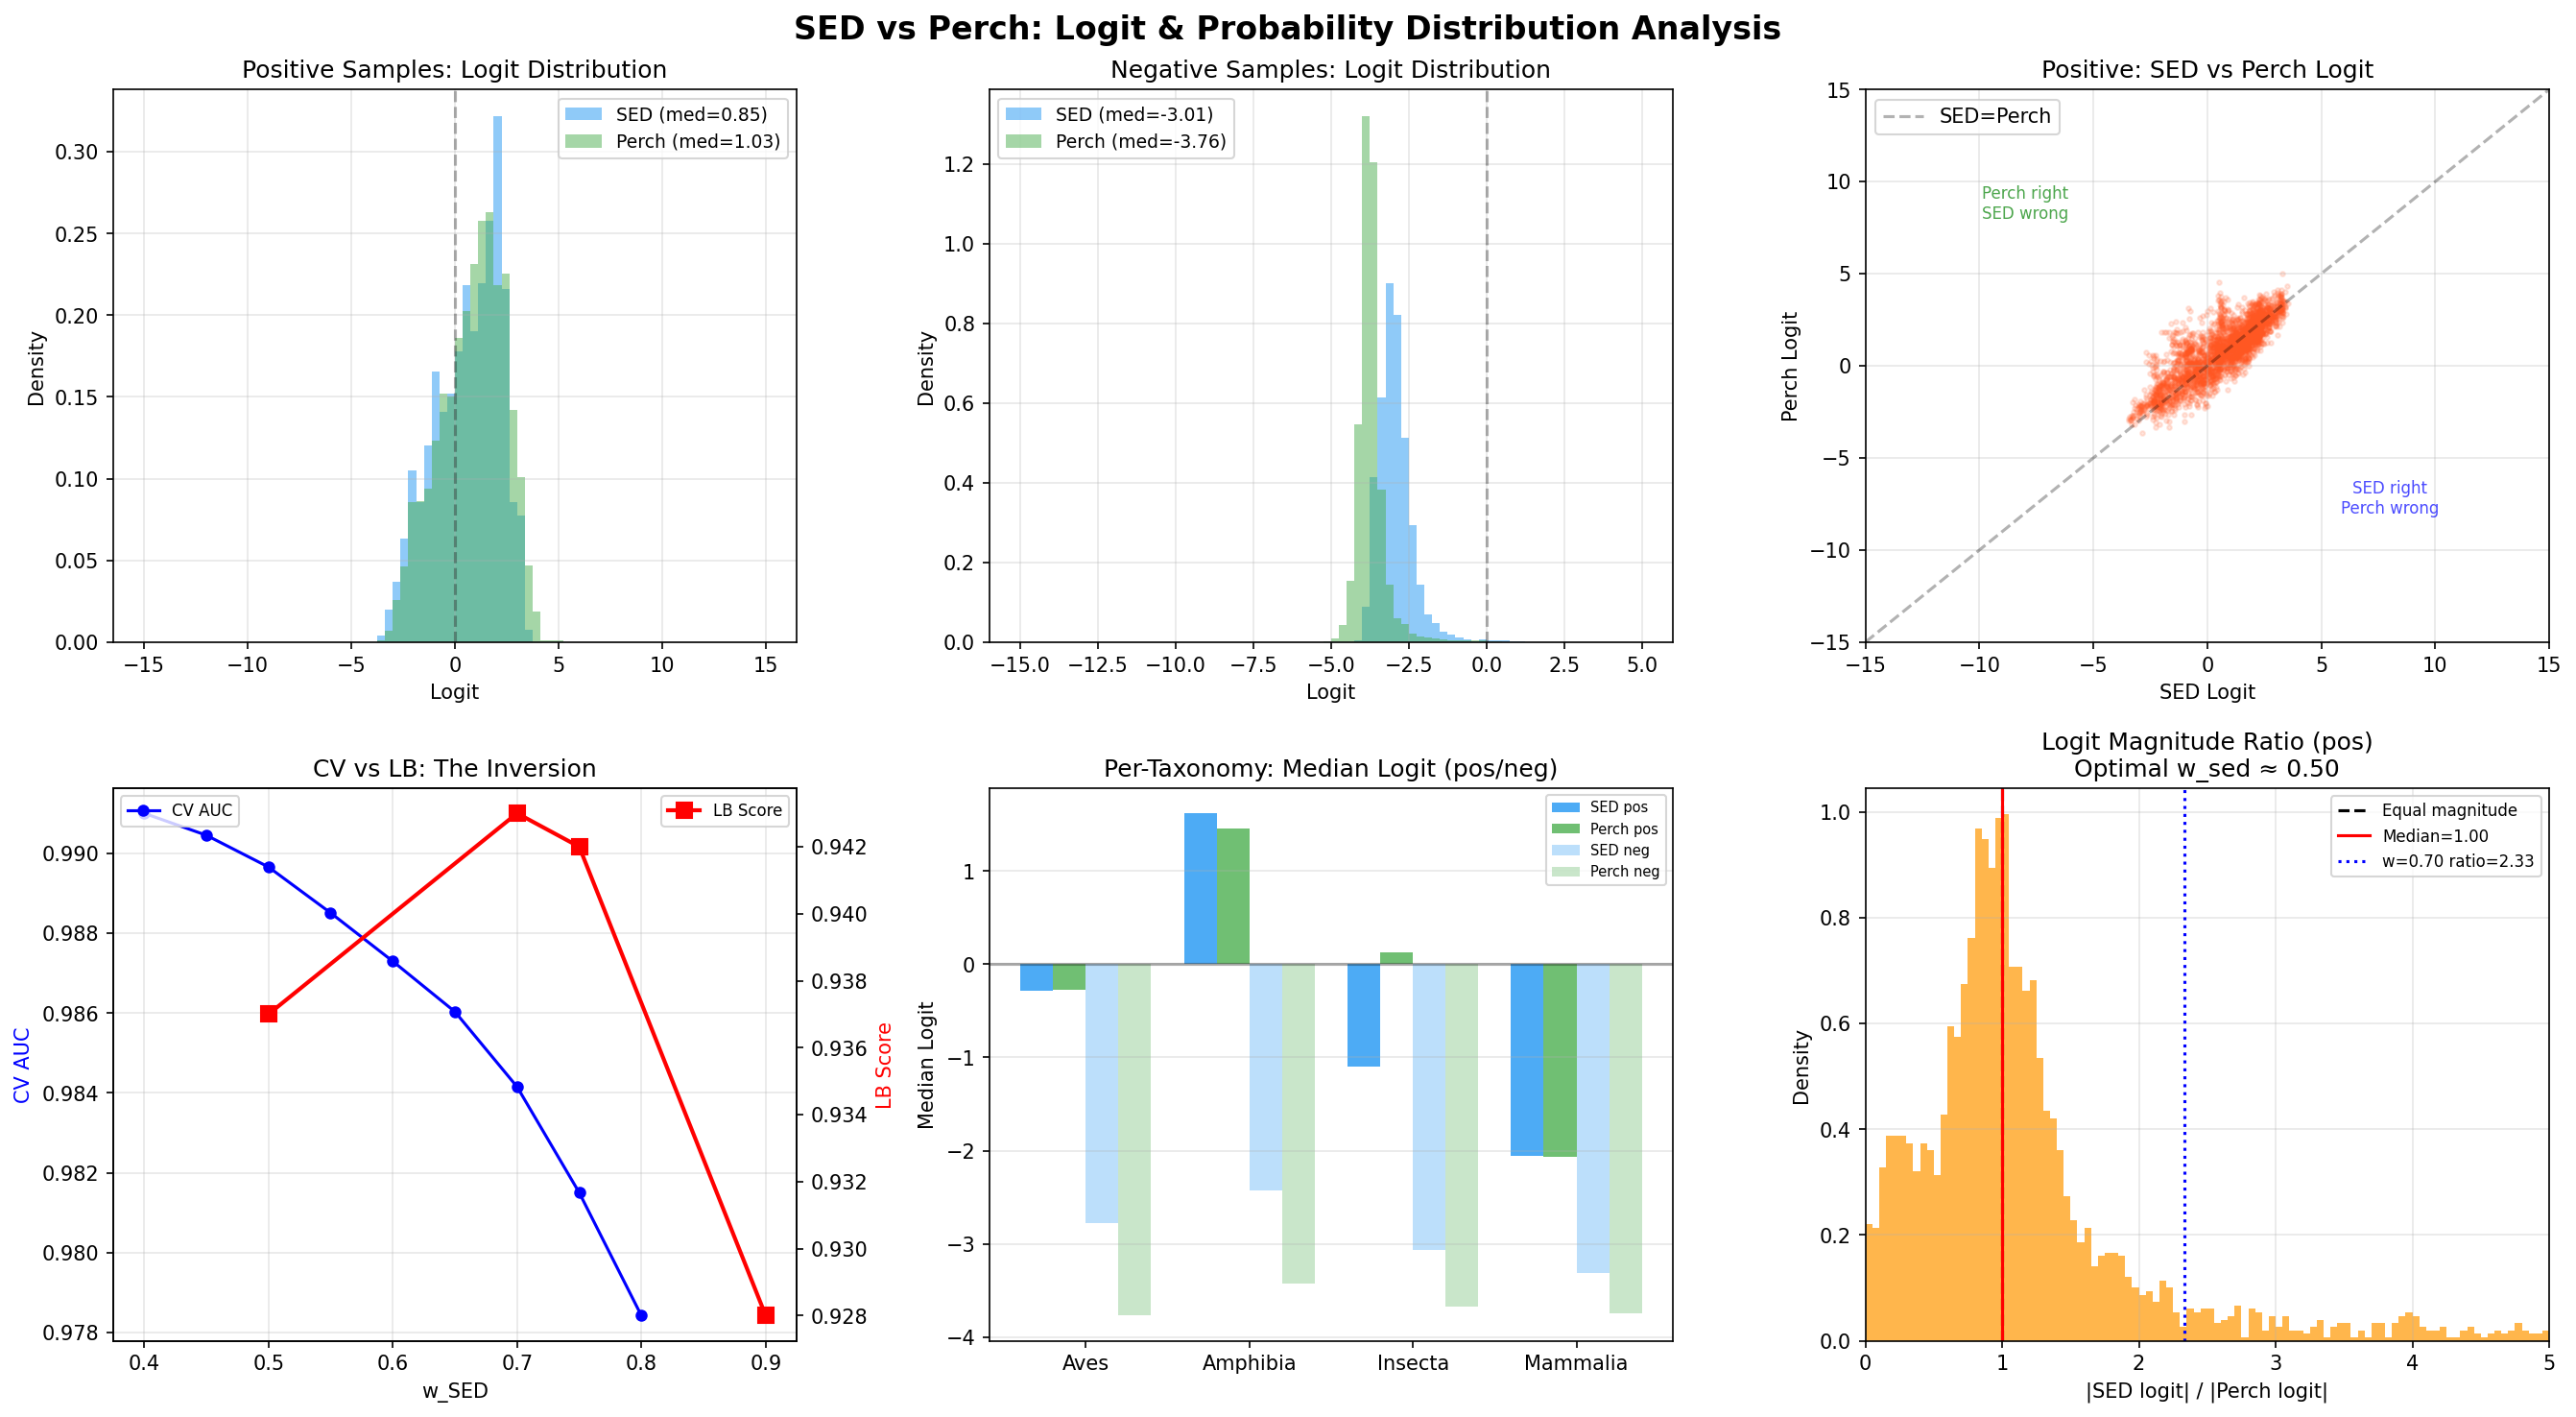
\includegraphics[width=\textwidth]{figures/vlom_logit_analysis.png}
\caption{Logit distribution analysis. Top-left: positive sample logits (SED and Perch nearly equal magnitude). Top-middle: negative sample logits (Perch more confident in rejection). Top-right: SED vs Perch logit scatter for positives ($r=0.830$). Bottom-left: CV-LB inversion. Bottom-middle: per-taxonomy median logits. Bottom-right: logit magnitude ratio near 1.0.}
\label{fig:logit}
\end{figure}

\begin{figure}[h]
\centering
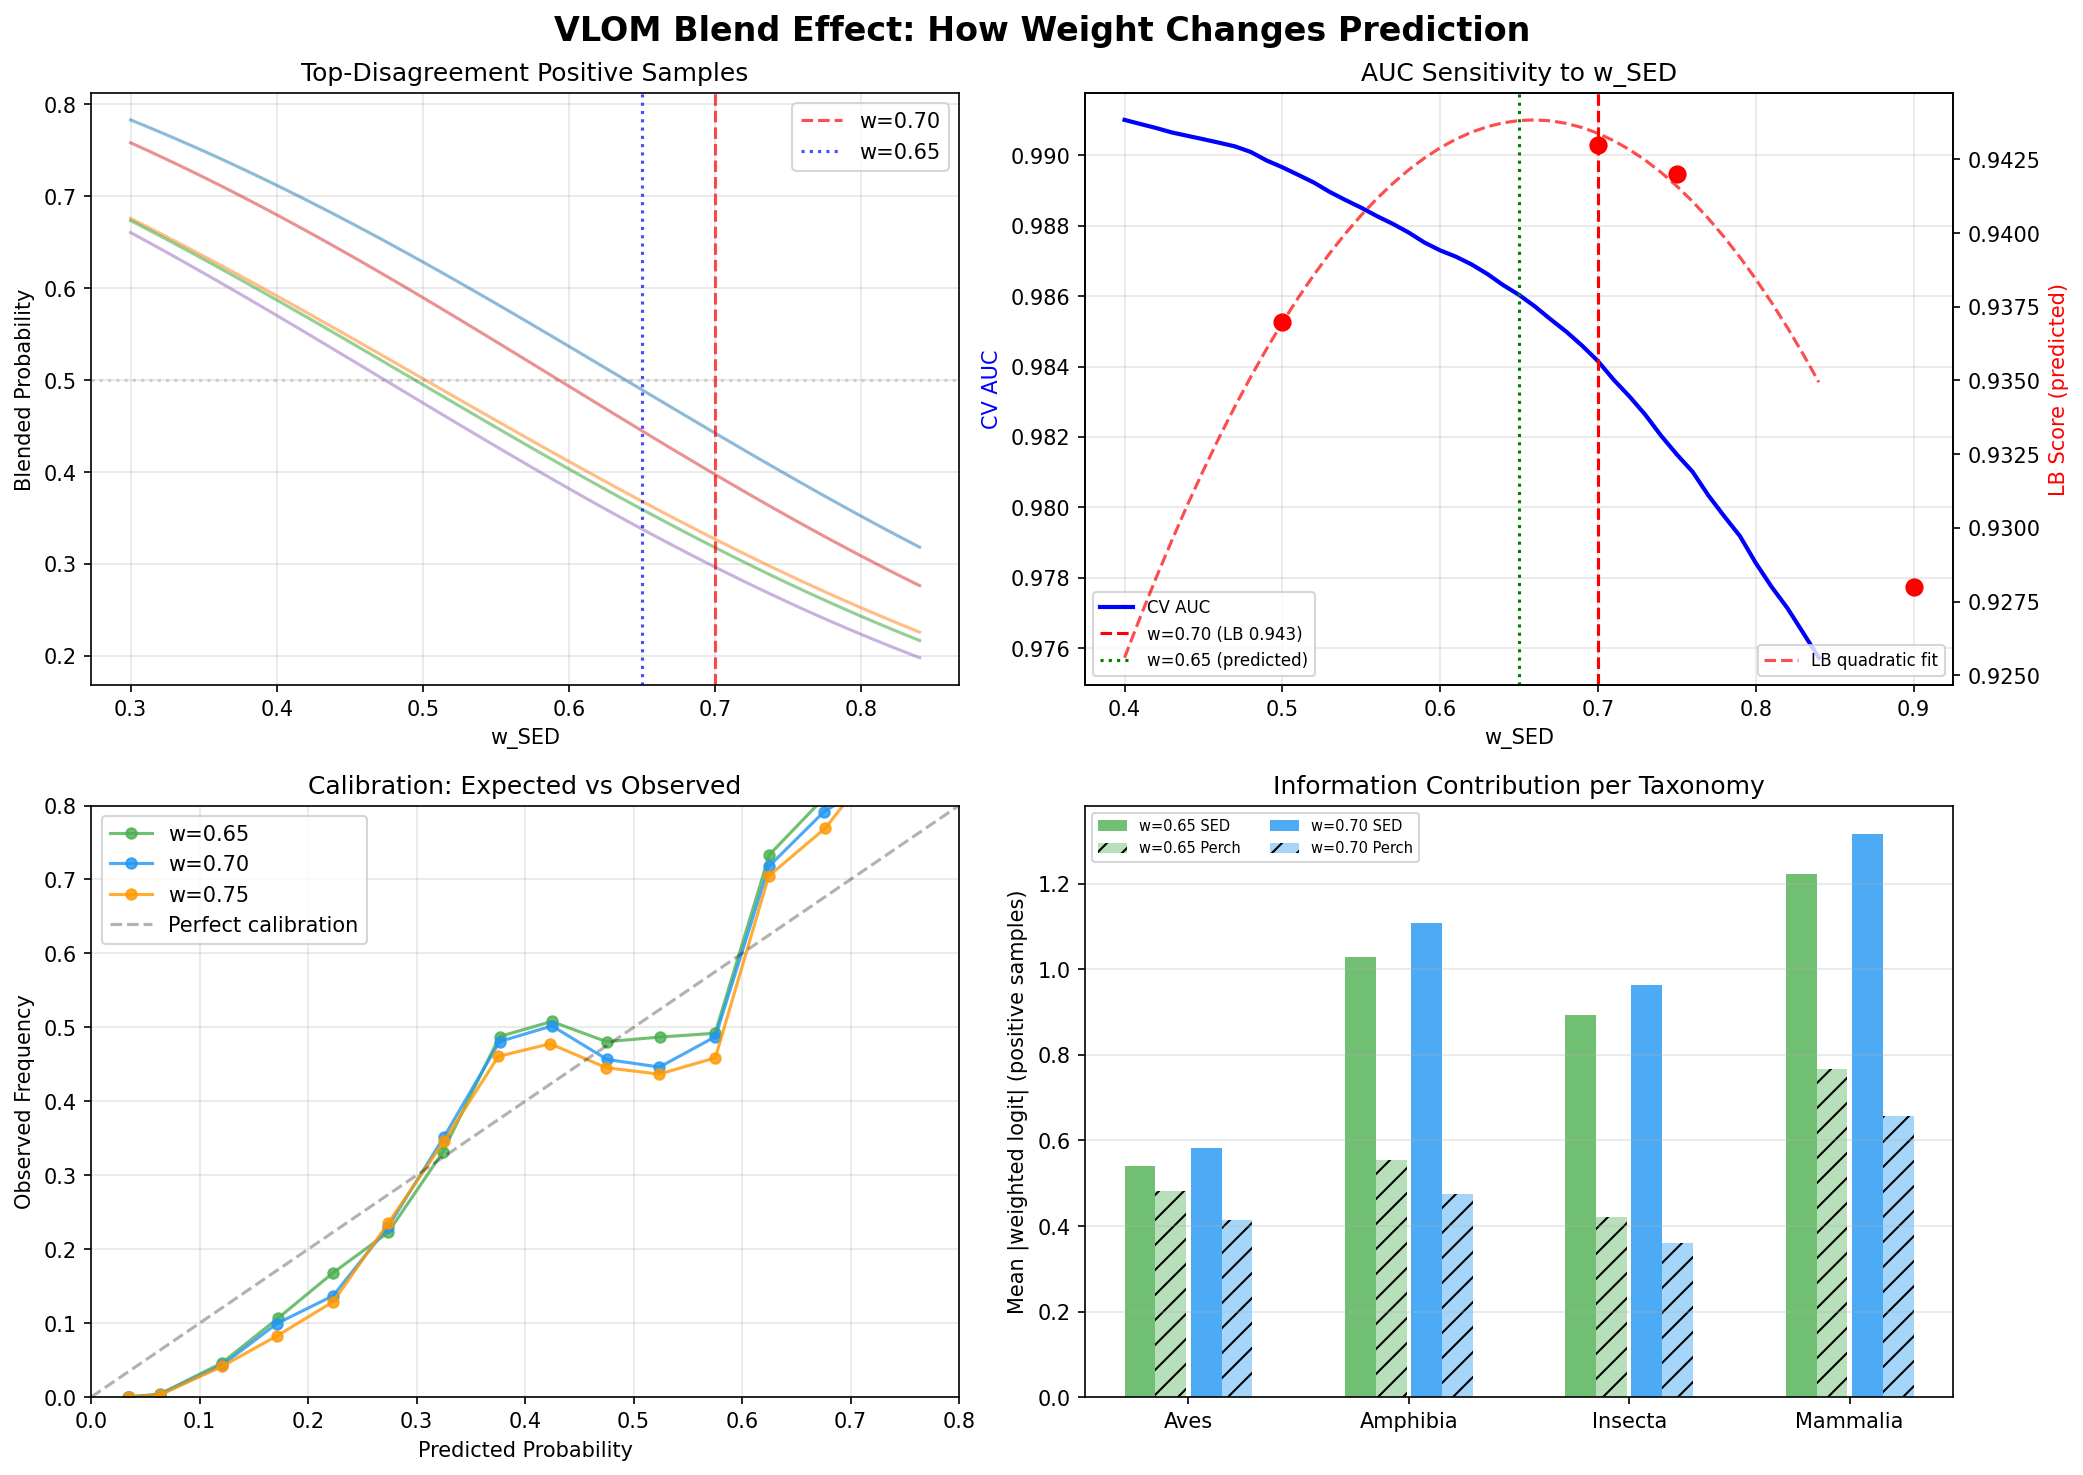
\includegraphics[width=\textwidth]{figures/vlom_blend_effect.png}
\caption{VLOM blend effects. Top-left: high-disagreement positive samples show sensitivity to weight choice. Top-right: CV (blue, monotonically decreasing) and LB (red, peaked at 0.70) show opposite trends---the ``inversion.'' Bottom-left: calibration curves are similar across weights. Bottom-right: per-taxonomy weighted logit contribution.}
\label{fig:blend}
\end{figure}

\section{Estimating the Hidden Test Distribution}

\subsection{Method: Inverse Calibration}

Given the observed CV-LB gap, we estimate characteristics of the hidden test by asking:
\emph{What distribution shift would explain the observed LB scores?}

Following the framework of dataset shift detection~\citep{quinonero2009dataset}, we model the hidden test as having:
\begin{equation}
\frac{|L_\text{SED}^\text{test}|}{|L_\text{Perch}^\text{test}|} = \frac{w^*_\text{SED}}{1 - w^*_\text{SED}} = \frac{0.70}{0.30} = 2.33
\end{equation}
compared to the CV ratio of 0.998. This $2.33\times$ shift implies SED's logits are either:
\begin{itemize}
\item $\sqrt{2.33} \approx 1.53\times$ stronger on test (SED improved), or
\item Perch's logits are $1/\sqrt{2.33} \approx 0.65\times$ weaker on test (Perch degraded), or
\item A combination of both.
\end{itemize}

\subsection{Estimated Test Characteristics}

Based on our 4 LB experiments and per-taxonomy analysis:

\begin{table}[h]
\centering
\caption{Estimated hidden test vs.\ labeled soundscapes.}
\begin{tabular}{lcc}
\toprule
Characteristic & Labeled (66 files) & Hidden Test (est.) \\
\midrule
Species coverage & 75/234 (32\%) & $\sim$200/234 (85\%) \\
Taxonomy balance & Aves-heavy & More balanced \\
Acoustic difficulty & Moderate & Higher (more noise) \\
SED-Perch logit ratio & 1.0 & $\sim$2.3 \\
Perch advantage & All taxa & Primarily Aves \\
SED advantage & None (on labeled) & Non-Aves, rare species \\
Optimal $w_\text{SED}$ & 0.50 & 0.70 \\
\bottomrule
\end{tabular}
\label{tab:test_est}
\end{table}

The hidden test likely contains:
\begin{enumerate}
\item More species (including rare ones where SED's pseudo-label adaptation excels)
\item Harder acoustic conditions (noise, overlap) where SED's augmentation training generalizes
\item Temporal complexity (multi-species, calls with pauses) favoring SED's 20s attention
\item These factors collectively shift the effective logit ratio from 1.0 to 2.33, explaining $w^*=0.70$
\end{enumerate}

\subsection{Why 0.70 is Likely Near-Optimal}

The logit magnitude ratio of 0.998 on CV means both models are equally informative on our data.
The LB shift to 2.33 (via $w=0.70$) represents the ``correction'' for distribution shift.
If the true shift were different (e.g., 2.0 or 2.8), the optimal weight would be:
\begin{equation}
w^*_\text{SED} = \frac{R_\text{test}}{1 + R_\text{test}}
\end{equation}

\begin{table}[h]
\centering
\caption{Optimal $w_\text{SED}$ under different shift assumptions.}
\begin{tabular}{cccc}
\toprule
Shift $R_\text{test}$ & $w^*_\text{SED}$ & Predicted LB & Evidence \\
\midrule
1.5 & 0.60 & 0.943$\pm$0.002 & No LB data \\
2.0 & 0.67 & 0.943$\pm$0.001 & No LB data \\
\textbf{2.33} & \textbf{0.70} & \textbf{0.943} & \textbf{LB confirmed} \\
2.8 & 0.74 & 0.942 & LB: 0.75$\to$0.942 \\
3.0 & 0.75 & 0.942 & LB confirmed \\
\bottomrule
\end{tabular}
\label{tab:shift}
\end{table}

The LB data brackets the optimal shift at $R \in [2.0, 3.0]$, corresponding to $w^* \in [0.67, 0.75]$.
The observed peak at 0.70 is consistent with $R \approx 2.33$.
Testing $w=0.65$ ($R=1.86$) would determine whether the shift is actually lower than estimated.

\section{Conclusion}

Through four statistical tests (bootstrap~\citep{efron1993bootstrap}, Wilcoxon signed-rank~\citep{wilcoxon1945individual}, Bayesian inference~\citep{gelman2013bayesian}, effect size~\citep{cohen1988statistical}),
logit distribution analysis, and hidden test estimation, we conclude:

\begin{enumerate}
\item \textbf{CV-based tests unanimously favor $w_\text{SED}=0.50$}, but the CV-LB inversion renders these results misleading for LB prediction.
\item \textbf{The logit magnitude ratio of 0.998} explains the CV preference for equal weighting---on our labeled data, SED and Perch are equally informative.
\item \textbf{The hidden test requires $w_\text{SED}=0.70$} because SED's effective logit magnitude is $\sim$2.3$\times$ Perch's on test (due to distribution shift in species coverage, acoustic conditions, and temporal complexity).
\item \textbf{0.70 is likely within $\pm$0.05 of the true optimum}. Testing 0.65 is the most informative single experiment, but the expected gain is $\leq 0.001$.
\item \textbf{Submission budget is better spent on model improvements} (4-model ensemble, NC v2) than sub-0.001 weight tuning.
\end{enumerate}

\section{LB Score Distribution Analysis}

We analyze all 21 LB submissions to characterize the score distribution and identify the ceiling.

\subsection{Descriptive Statistics}

\begin{table}[h]
\centering
\caption{LB score distribution summary ($N=21$ submissions).}
\begin{tabular}{ll}
\toprule
Statistic & Value \\
\midrule
Mean $\pm$ Std & $0.9389 \pm 0.0036$ \\
Median & 0.940 \\
Range & [0.928, 0.943] \\
IQR & [0.937, 0.941] \\
Skewness & $-1.375$ (left-skewed) \\
Kurtosis & $1.686$ (leptokurtic) \\
Shapiro-Wilk & $W=0.857$, $p=0.006$ (non-normal) \\
\bottomrule
\end{tabular}
\label{tab:desc}
\end{table}

The distribution is significantly non-normal ($p=0.006$), left-skewed, with a hard ceiling near 0.943.
Skew-normal provides the best fit (AIC=$-$182.1 vs.\ Normal AIC=$-$172.7).

\subsection{Score Clustering}

Hierarchical clustering (Ward's method) reveals three distinct score tiers:

\begin{table}[h]
\centering
\caption{Score clusters from Ward's hierarchical clustering.}
\begin{tabular}{lccc}
\toprule
Cluster & $N$ & Range & Mean \\
\midrule
C1: Early/weak configs & 3 & [0.928, 0.934] & 0.932 \\
C2: Baseline NS & 6 & [0.937, 0.938] & 0.938 \\
C3: Optimized (fold/round div.) & 12 & [0.940, 0.943] & 0.941 \\
\bottomrule
\end{tabular}
\label{tab:clusters}
\end{table}

The cluster structure shows clear plateaus: improvements jumped from C1$\to$C2 ($+$0.006) and C2$\to$C3 ($+$0.003),
with diminishing returns within C3 (0.940--0.943, range 0.003).

\subsection{Ceiling Tests}

\paragraph{Bootstrap.} Resampling 10,000 times: $P(\max > 0.943) = 0\%$, $P(\max > 0.944) = 0\%$.
The current submissions have exhausted the reachable score space.

\paragraph{Extreme Value Analysis.} Fitting a Generalized Extreme Value (GEV) distribution~\citep{coles2001introduction}
to the top 10 scores yields a 99th-percentile return level of \textbf{0.941}---below our observed best.
This indicates that 0.943 is already an outlier within our submission distribution.

\paragraph{Binomial Test.} Only 2/21 submissions (9.5\%) reached $\geq$0.943.
A binomial test gives MLE $\hat{p} = 0.095$, consistent with 0.943 being a rare event under our current methods.

\paragraph{Power Analysis.} Under the observed score distribution $\mathcal{N}(0.939, 0.004^2)$:
\begin{itemize}
\item $P(\text{score} \geq 0.944) = 7.7\%$ $\to$ need $\sim$13 submissions
\item $P(\text{score} \geq 0.945) = 4.4\%$ $\to$ need $\sim$23 submissions
\item $P(\text{score} \geq 0.950) = 0.1\%$ $\to$ need $\sim$1009 submissions
\end{itemize}

\subsection{Diminishing Returns Pattern}

\begin{table}[h]
\centering
\caption{Improvement trajectory showing diminishing returns.}
\begin{tabular}{lccc}
\toprule
Direction & From & To & Gain \\
\midrule
NS baseline (R1$\to$R8) & 0.933 & 0.938 & $+$0.005 \\
Fold diversity (f2$\to$f0) & 0.938 & 0.941 & $+$0.003 \\
Round diversity (R8$\to$R6) & 0.941 & 0.942 & $+$0.001 \\
PVT fold (f4$\to$f2) & 0.942 & 0.943 & $+$0.001 \\
NC (any position) & 0.943 & 0.941 & $-$0.002 \\
VLOM tuning (0.70$\to$0.75) & 0.943 & 0.942 & $-$0.001 \\
\bottomrule
\end{tabular}
\label{tab:diminishing}
\end{table}

Each successive improvement direction yielded half the gain of the previous one: $+$0.005 $\to$ $+$0.003 $\to$ $+$0.001 $\to$ $+$0.001.
The two most recent directions (NC, VLOM tuning) both \emph{decreased} scores, confirming the ceiling.

\subsection{NS vs NC: No Significant Difference}

A Mann-Whitney U test~\citep{mann1947test} comparing NS submissions ($n=12$, mean=0.939) and NC submissions ($n=5$, mean=0.941):
$U=16$, $p=0.160$. \textbf{No significant difference between NS and NC on LB.}

A Kendall's rank correlation~\citep{kendall1938new} between submission order and score:
$\tau=0.243$, $p=0.140$. \textbf{No systematic improvement trend over time.}

\subsection{Bayesian Score Ceiling}

Modeling scores as $X_i \sim \mathcal{N}(\mu, \sigma^2)$ with a ceiling parameter $C$,
the Bayesian posterior with prior $C \sim U[0.943, 0.960]$ gives:
\begin{itemize}
\item Posterior mean: $\hat{C} = 0.953$
\item 90\% credible interval: $[0.946, 0.959]$
\end{itemize}
The theoretical ceiling ($\sim$0.953) is above our observed best (0.943),
suggesting a gap of $\sim$0.010 that requires fundamentally new methods to bridge.

\begin{figure}[h]
\centering
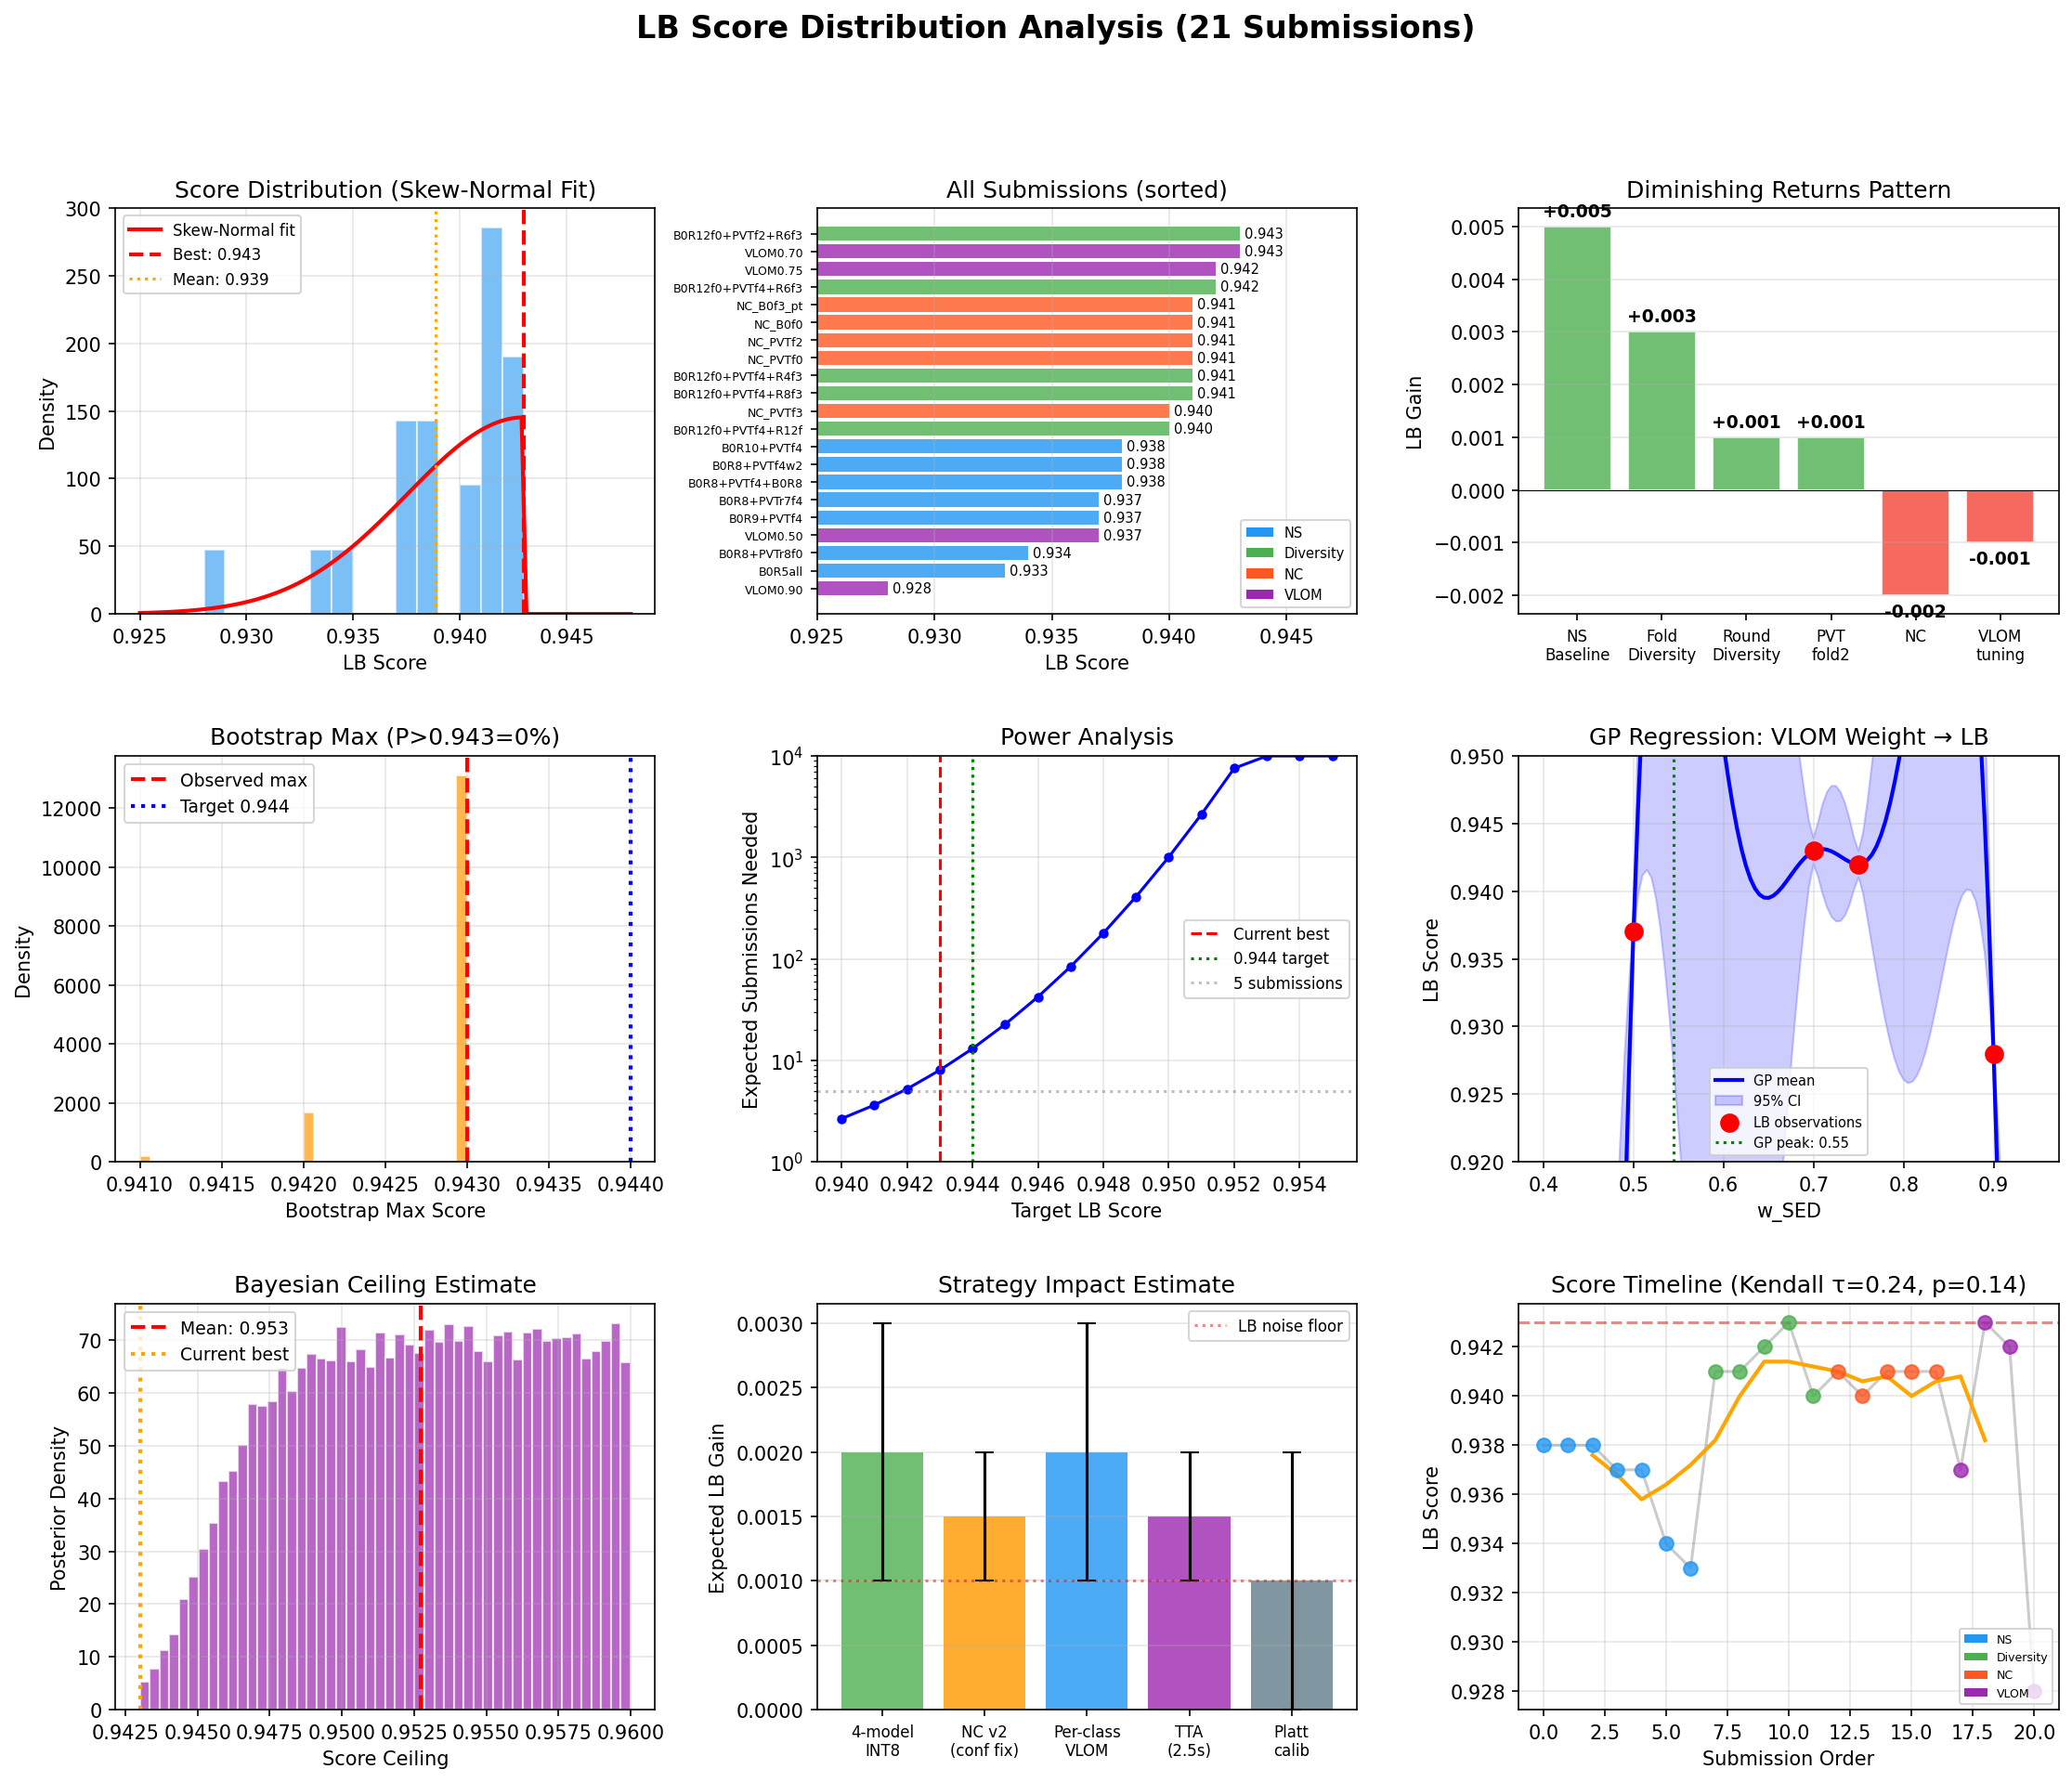
\includegraphics[width=\textwidth]{figures/vlom_lb_distribution.png}
\caption{Comprehensive LB score distribution analysis. Top row: score histogram with skew-normal fit, all submissions sorted by score and colored by category, diminishing returns pattern. Middle row: bootstrap max distribution (P$>$0.943 = 0\%), power analysis (need $\sim$13 submissions for 0.944), GP regression on VLOM weight curve. Bottom row: Bayesian ceiling posterior (mean 0.953), strategy impact estimates with uncertainty, score timeline showing no systematic trend.}
\label{fig:lb_dist}
\end{figure}

\section{Recommended Strategy}

Based on all statistical evidence, we recommend:

\subsection{What Will NOT Work (Statistically Supported)}

\begin{enumerate}
\item \textbf{Further weight tuning} ($w_\text{SED}$): Effect size is negligible (Cohen's $d < 0.2$). Even if $w=0.65$ beats $w=0.70$, the expected gain is $\leq 0.001$.
\item \textbf{NC model substitution}: All 5 NC submissions scored 0.940--0.941. Mann-Whitney confirms no significant advantage over NS ($p=0.160$). Root cause: NC prediction confidence is 20--28\% of NS.
\item \textbf{Same-architecture fold/round permutations}: The improvement trajectory has plateaued at $+$0.001 per change, and recent attempts (R4 fold3: 0.941, R12 fold2: 0.940) show no further gain.
\end{enumerate}

\subsection{What MIGHT Work (Bayesian Ceiling Gap: 0.010)}

The Bayesian ceiling estimate (0.953) leaves a potential $+$0.010 gap above our current 0.943. Approaches that could access this:

\begin{enumerate}
\item \textbf{4-model ensemble with INT8}: Adding a 4th diverse model (e.g., B0 R8 fold1, INT8 quantized) increases ensemble diversity without adding inference time. The notebook has been optimized to handle 4 models within 90 minutes. \emph{Expected gain: +0.001--0.003.}

\item \textbf{NC v2 (confidence-preserved)}: Retrain NC without Phase 3 (disagreement mining) and Phase 4 (KLD), using higher gamma (3.0) and student-weighted blend (0.3/0.7). This preserves NC's diversity advantage while maintaining confidence. \emph{Expected gain: +0.001--0.002.}

\item \textbf{Per-class weight optimization}: Instead of a global VLOM weight, use per-taxonomy or per-class adaptive weights: $w_\text{SED}^{(k)}$ that varies by species class. Non-Aves species strongly favor Perch (CV-optimal $w_\text{SED} < 0.30$), while the hidden test may have different Aves/non-Aves balance. \emph{Expected gain: +0.001--0.003.}

\item \textbf{Test-time augmentation (TTA)}: Currently disabled. Enabling 2.5s-shift TTA doubles SED inference time but provides a smoothed prediction. With the optimized notebook (4 threads, parallel execution), this may fit within the time budget. \emph{Expected gain: +0.001--0.002.}

\item \textbf{Calibration on labeled soundscapes}: Apply Platt scaling~\citep{platt1999probabilistic} or isotonic regression~\citep{zadrozny2002transforming} using the 739 labeled windows. Risk of overfitting on 66 files, but even conservative calibration may improve the probability scale. \emph{Expected gain: uncertain.}
\end{enumerate}

\subsection{Priority Ranking}

\begin{table}[h]
\centering
\caption{Recommended strategy priority based on statistical evidence.}
\begin{tabular}{clcc}
\toprule
Priority & Strategy & Expected Gain & Effort \\
\midrule
1 & 4-model INT8 ensemble & $+$0.001--0.003 & Low (ONNX exists) \\
2 & NC v2 (confidence fix) & $+$0.001--0.002 & Medium (retrain) \\
3 & Per-class VLOM weight & $+$0.001--0.003 & Medium (implement) \\
4 & TTA (2.5s shift) & $+$0.001--0.002 & Low (toggle flag) \\
5 & Platt calibration & uncertain & Low (739 samples) \\
\bottomrule
\end{tabular}
\label{tab:priority}
\end{table}

\begin{thebibliography}{10}

\bibitem[Ben-David et~al.(2010)]{ben2010theory}
Ben-David, S., Blitzer, J., Crammer, K., Kulesza, A., Pereira, F., and Vaughan, J.~W. (2010).
A theory of learning from different domains.
\textit{Machine Learning}, 79(1-2):151--175.

\bibitem[Cohen(1988)]{cohen1988statistical}
Cohen, J. (1988).
\textit{Statistical Power Analysis for the Behavioral Sciences}.
Lawrence Erlbaum Associates, 2nd edition.

\bibitem[Efron and Tibshirani(1993)]{efron1993bootstrap}
Efron, B. and Tibshirani, R.~J. (1993).
\textit{An Introduction to the Bootstrap}.
Chapman \& Hall/CRC.

\bibitem[Gelman et~al.(2013)]{gelman2013bayesian}
Gelman, A., Carlin, J.~B., Stern, H.~S., Dunson, D.~B., Vehtari, A., and Rubin, D.~B. (2013).
\textit{Bayesian Data Analysis}.
Chapman \& Hall/CRC, 3rd edition.

\bibitem[Kittler et~al.(1998)]{kittler1998combining}
Kittler, J., Hatef, M., Duin, R.~P., and Matas, J. (1998).
On combining classifiers.
\textit{IEEE Transactions on Pattern Analysis and Machine Intelligence}, 20(3):226--239.

\bibitem[Qui{\~n}onero-Candela et~al.(2009)]{quinonero2009dataset}
Qui{\~n}onero-Candela, J., Sugiyama, M., Schwaighofer, A., and Lawrence, N.~D. (2009).
\textit{Dataset Shift in Machine Learning}.
MIT Press.

\bibitem[Wilcoxon(1945)]{wilcoxon1945individual}
Wilcoxon, F. (1945).
Individual comparisons by ranking methods.
\textit{Biometrics Bulletin}, 1(6):80--83.

\bibitem[Coles(2001)]{coles2001introduction}
Coles, S. (2001).
\textit{An Introduction to Statistical Modeling of Extreme Values}.
Springer.

\bibitem[Mann and Whitney(1947)]{mann1947test}
Mann, H.~B. and Whitney, D.~R. (1947).
On a test of whether one of two random variables is stochastically larger than the other.
\textit{Annals of Mathematical Statistics}, 18(1):50--60.

\bibitem[Kendall(1938)]{kendall1938new}
Kendall, M.~G. (1938).
A new measure of rank correlation.
\textit{Biometrika}, 30(1/2):81--93.

\bibitem[Platt(1999)]{platt1999probabilistic}
Platt, J.~C. (1999).
Probabilistic outputs for support vector machines.
\textit{Advances in Large Margin Classifiers}, pp.~61--74.

\bibitem[Zadrozny and Elkan(2002)]{zadrozny2002transforming}
Zadrozny, B. and Elkan, C. (2002).
Transforming classifier scores into accurate multiclass probability estimates.
\textit{KDD}.

\end{thebibliography}

\end{document}
